\subsection{Configure GBTx to use GBT-IC channel}
It might be useful to read/write individual registers from/to a GBTx board. In
this case, follow the \autoref{fig:gbt-ic} to flip the \texttt{configSelect}
switch.

\begin{leftbar}
    Flip the \texttt{configSelect} switch will render the external \itwoc
    adapter ineffective.
    None of the GBTx register value is fused onto the board, so a GBTx board in
    our lab must always be programmed externally via \itwoc before flipping the
    switch.
\end{leftbar}

\begin{center}
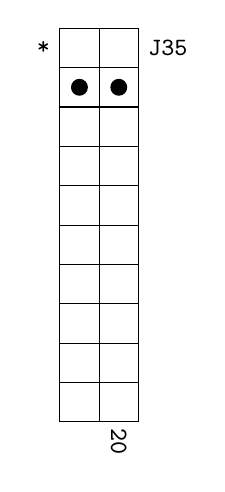
\begin{tikzpicture}
    % Pins
    \draw (0,0) rectangle (1,-5);
    \draw (0.5,0) to (0.5,-5);
    \draw (0,-0.5) to (1,-0.5);
    \draw (0,-1.5) to (1,-1.5);
    \draw (0,-2.5) to (1,-2.5);
    \draw (0,-3.5) to (1,-3.5);
    \draw (0,-4.5) to (1,-4.5);
    \draw (0,-1) to (1,-1);
    \draw (0,-2) to (1,-2);
    \draw (0,-3) to (1,-3);
    \draw (0,-4) to (1,-4);

    % PCB labels
    \coordinate (A) at (1,-0.25);
    \node at (A) [right] {\small\texttt{J35}};
    \coordinate (B) at (0,-0.25);
    \node at (B) [left] {\small\texttt{*}};
    \coordinate (C) at (0.75,-5.25);
    \node at (C) [rotate=-90] {\small\texttt{20}};

    % Pins that need to be connected
    \draw [black,fill] (0.25,-0.75) circle [radius=0.1];
    \draw [black,fill] (0.75,-0.75) circle [radius=0.1];
\end{tikzpicture}
\captionof{figure}{
    Schematic for flipping the \texttt{configSelect} switch. A jumper should be
    used to connect the two pins marked above.
}
\label{fig:gbt-ic}
\end{center}
